\chapter{Ejercicio 1}
\part{Ejercicio 1}
\section{Enunciado}
Dado un n'umero natural n mayor que 1, encontrar el n'umero primo p que aparece con mayor potencia en la factorizaci'on de n. En caso de haber m'as de un n'umero primo con  la mayor potencia, encontrar el mayor de ellos.

%TODO: revisar la claridad de esto, ver si se puede mejorar
\section{Desarrollo}
La primer idea para resolver el ejercicio fue obtener los primos menores que el n'umero a factorizar
(en adelante $n$) y luego obtener la potencia con la que cada uno lo divide, qued'andonos con el de mayor
potencia o con el mayor de todos los de m'axima potencia. Sin embargo esta soluci'on era costosa, ya que requeria obtener primeramente todos aquellos primos que sean menores a $n$.
\paragraph{}
Un segundo acercamiento nos permiti'o salvar esta dificultad, de manera que no fue necesario obtener los primos menores a $n$ expl'icitamente. El proceso consiste en partir de 2, probar manualmente si 2, 3 y 5 dividen a $n$ y a partir  de aqu'i ciclar generando numeros de la forma $6*k + 1$ o $6*k + 5$ con $k \geq 1$ (se puede demostrar que los numeros primos mayores que 5 tienen esta forma. Ver Demostraci'on 1).
\paragraph{}
Cuando hallamos algun numero primo que divide a $n$, buscamos su multiplicidad dividiendo nuestro numero por dicho primo, las veces que sean posibles. Una vez calculada, se verifica si esta nueva multiplicidad es mayor a la guardada hasta el momento. Si lo es, esta es reemplazada por la nueva y se guarda. Una vez hecho esto se pasa al siguiente posible primo, repitiendo el proceso anterior pero ahora con un nuevo $n$ que llamaremos $n'$, que resulta de dividir $n$ por el numero primo, elevado a la potencia hallada. Este proceso se repite mientras nuestro proximo primo, no supere la raiz de $n'$. Un problema de este m'etodo es que se hacen divisiones por n'umeros que no son primos, pero su costo es menor comparandolo con otras metodologias que buscan todos los menores a $n$, o que verifican si dicho numero lo es antes de hacer la division.
\paragraph{}
Es importante notar que si un numero no es primo, este no puede dividir a $n$ (ver demostraci'on 2). Si no se pudiera asegurar esto, el algoritmo fallar'ia.
Un ejemplo simple seria al factorizar $30 = 2*3*5$. En este caso se guardar'ia a 15 como m'aximo factor primo, lo cual resulta claramente erroneo. Finalmente, utilizamos un teorema que nos dice que si un numero es compuesto existe por lo menos un primo menor que su raiz que lo divide (ver demostraci'on 3), de esta manera iteramos solo hasta la ra'iz del numero (la cual se actualiza luego de terminada la divisi'on) en vez de hasta $n$.

\section{Demostraciones}
\subsection{Teorema 1}
\paragraph{Enunciado:}
Sea p $\in$ $\enteros$, primo , p $>$ 5, entonces $\exists$ k $\in$ $\enteros$ $\geq$ 1  tal que p = $6*k+1$ o p = $6*k +5$.
\paragraph{Demostraci'on:}
Lo demostraremos por absurdo.\\ Supongamos que $\exists$ p $\in$ $\enteros$, primo, tal que p $>$ 5 y p $\not\equiv$ 1  $\mod{6}$ y p
$\not\equiv$ 5  $\mod{6}$, luego p = $6*k + j$ con j $\in$ ${0,2,3,4}$ \\
si $j = 0$\\
$6*k$ $\equiv$ 0  $\mod{6}$, absurdo pues p es primo\\
si $j = 2$\\
$6*k + 2$ $\equiv$ 0  $\mod{2}$, absurdo pues p es primo \\
si $j = 3$\\
$6*k + 3$ $\equiv$ 0  $\mod{3}$, nuevamente absurdo\\
si $j = 4$\\
$6*k + 4$ $\equiv$ 0  $\mod{2}$, tambi'en llegamos a un absurdo.\\
Ergo, si p es primo y p $>$ 5, entonces p = $6*k+1$ o p = $6*k +5$

\subsection{Teorema 2}
\paragraph{Enunciado:}
Sea k $\in$ $\enteros$ compuesto, y sea n $\entero$ para todo p $\entero$, primo, p $<$ k, $(n:p) = 1$, entonces n $\not\equiv$ 0 $\mod{k}$
\paragraph{Demostraci'on}
Dado que k es compuesto existen $q_1,\ldots,q_j$ con $q_i$ primo tal que $q_1*\ldots*q_j = k$ \\
Supongamos que n $\equiv$ 0 $\mod{k}$,\\
Entonces como los $q_i$ son primos, vale que n $\equiv$ 0 $\mod{q_1}$ 'o ... 'o $n \equiv 0 \mod{q_j}$ \\
Pero sabemos que $q_i < k$ y que por lo tanto $(n:q_{i}) = 1$ \\
Llegamos entonces a un absurdo que provino de suponer que  $n \equiv 0 \mod{k}$ \\ 
Luego $n \not\equiv 0 \mod{k}$, que era lo que queriamos probar

\subsection{Teorema 3}
\paragraph{Enunciado:}
$k$ $\entero$, $k>1$; $k$ es compuesto $\longleftrightarrow$ $\exists p$ ,primo, tal que $p \leq \sqrt{k}$ y $k \equiv 0 \mod{p}$ \\
\paragraph{Demostracion:}
$\leftarrow)$ trivial \\
$\rightarrow$) Como $k$ es compuesto se puede factorizar como $p_1*...*p_n$ con $p_i > \sqrt{k} \forall i \in {1...n}$\\
Entonces \\
$k = p_1*...*p_n > (\sqrt{k})^2*T$ , con $T>1$\\  
$k = p_1*...*p_n > \sqrt{k}^2*T$ pero $k*T > k$ \\
Absurdo, que provino de suponer que $p_i > \sqrt{k}$ $\forall i \in {1...n}$\\

%todo hacer el cambio al pseudocodigo para q sea mas facil la demo
\section{Pseudocodigo}
\begin{algorithm}
\caption{Halla $mejorPrimo$ y $mejorPotencia$}
\begin{algorithmic}[1]
\STATE $mejorPrimo \leftarrow 1$
\STATE $mejorPotencia \leftarrow 0$
\STATE $primoActual \leftarrow generar\_candidato()$
\STATE $potenciaActual \leftarrow 0$
\STATE $l \leftarrow limite(n)$
\WHILE{$n \neq 1$ $\&$ $primoActual \leq l$}
    \IF{$primoActual$  $|$ $n$}
        \STATE $potenciaActual++$
        \STATE $n \leftarrow n/primoActual$
    \ELSE
        \IF{$potenciaActual \geq mejorPotencia$}
            \STATE $mejorPrimo \leftarrow primoActual$
            \STATE $mejorPotencia \leftarrow potenciaActual$
        \ENDIF

        \STATE $potenciaActual \leftarrow 0$
        \STATE $primoActual \leftarrow generar\_candidato()$
        \STATE $l \leftarrow limite(n)$
    \ENDIF
\ENDWHILE
\IF{$primoActual > l$}
    \STATE $primoActual \leftarrow n$
    \STATE $potenciaActual \leftarrow 1$
\ENDIF
\IF{$potenciaActual \geq mejorPotencia$}
    \STATE $mejorPrimo \leftarrow primoActual$
    \STATE $mejorPotencia \leftarrow potenciaActual$
\ENDIF
\end{algorithmic}
\end{algorithm}


%TODO: hablar del calculo de complejidad, de porq logaritmico, hacer el calculo
%TODO: analisis de peor caso!
\section{C'alculo de complejidad}

%TODO: hablar de que sabemos q n no es tam de entrada, que dejamos los graficos porq se ve bien el o(sqrtn), ojo con esto q me parece q es O(raiz*log^3)
\section{Analisis Experimental}
\subsection{Experiencias realizadas}
Para el analisis del algoritmo decidimos medir tanto operaciones como tiempo. Primero medimos dichas variables para los numeros entre 2 y 100000 para observar un patron de comportamiento. A partir de esta experiencia, decidimos realizar otras dos, donde separamos numeros primos en una de ellas, y en otra tomamos las potencias de un primo (en particular de 7). Esto lo hicimos por considerar que el peor caso del algoritmo es precisamente cuando el numero es primo, mientras que el mejor es cuando el numero es potencia de un primo. Por otro lado realizamos experiencias similares pero teniendo en cuenta no el numero, sino la cantidad de bits que lo representan, es decir teniendo en cuenta el tama\~{n}o de la entrada. Para estas experriencias tomamos distintos numeros pero medimos la cantidad de operaciones y el tiempo, pero no para un n. sino para $floor(log_2(n)) + 1$ 
%TODO: hacer los graficos de tamanio que no estan
%TODO: revisar los graficos, tratar de q las leyendas se vean bien.
\subsection{Gr'aficos}
\begin{figure}[H]
\centering
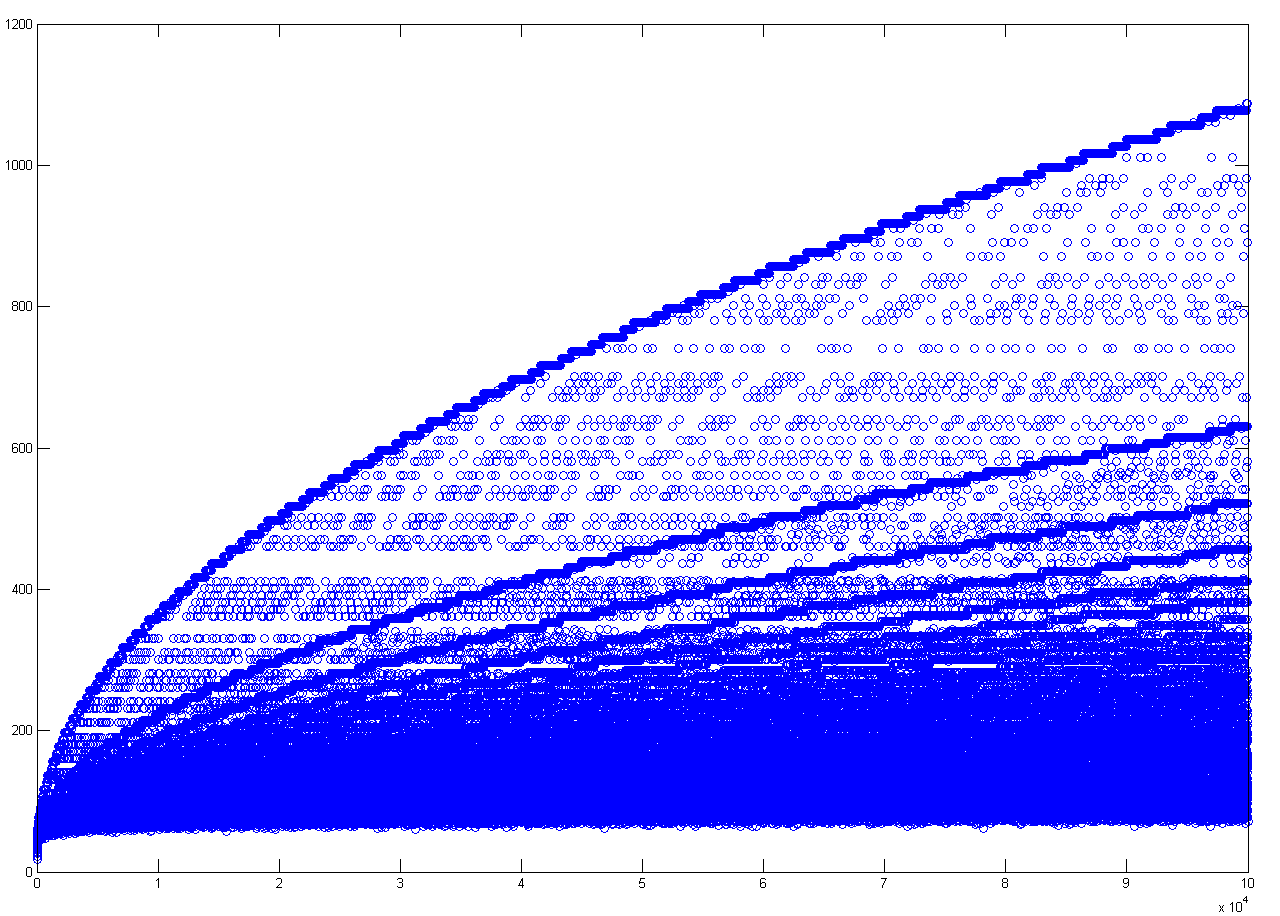
\includegraphics[scale=0.8]{../../codigo/ejercicio1/benchmark/graficos/todos_los_numeros/graficosTodos.png}
\caption{Cantidad de operaciones en funcion del n'umero}
\end{figure}

\begin{figure}[H]
\centering
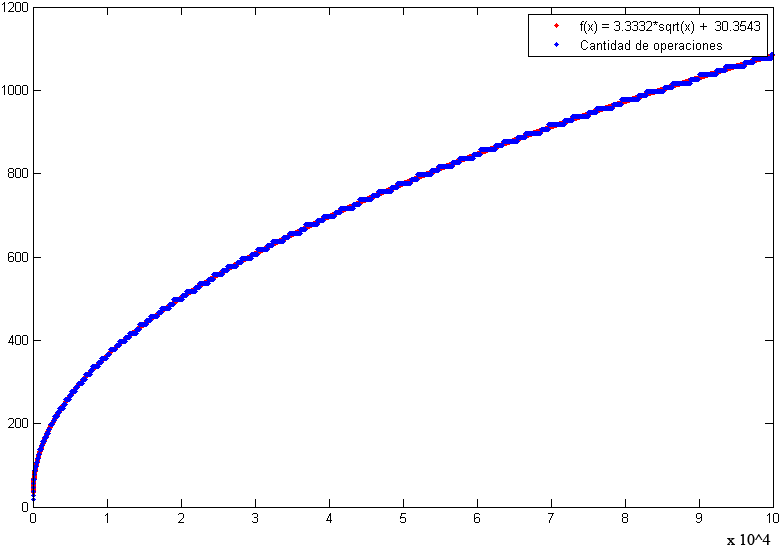
\includegraphics[scale=0.8]{../../codigo/ejercicio1/benchmark/graficos/primos/graficoPrimos.png}
\caption{Cantidad de operaciones en funcion del n'umero para n'umeros primos}
\end{figure}

\begin{figure}[H]
\centering
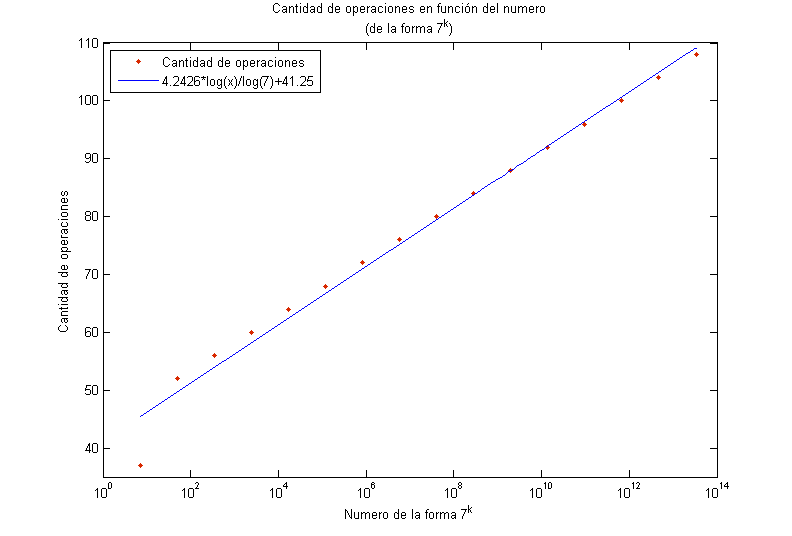
\includegraphics[scale=0.8]{../../codigo/ejercicio1/benchmark/graficos/potencias_de_7/graficoPotenciasDe7.png}
\caption{Cantidad de operaciones en funcion del n'umero para n'umeros de la forma $7^k$}
\end{figure}

\begin{figure}[H]
\centering
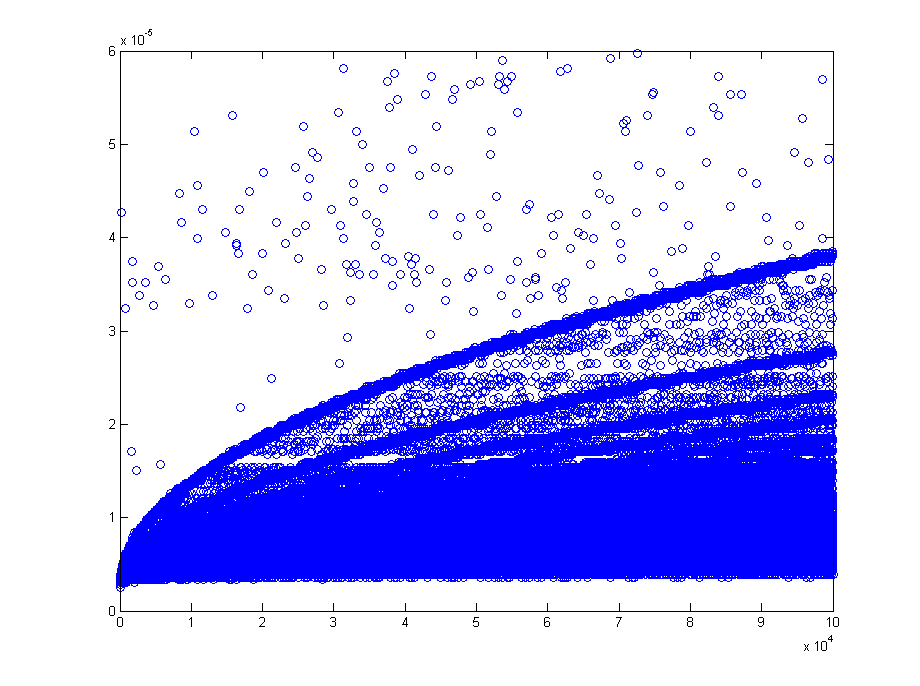
\includegraphics[scale=0.5]{../../codigo/ejercicio1/benchmark_de_tiempo/graficos/todos_los_numeros/todosLosNumerosPuntosTiempo.png}
\caption{Tiempo en funcion del n'umero}
\end{figure}

\begin{figure}[H]
\centering
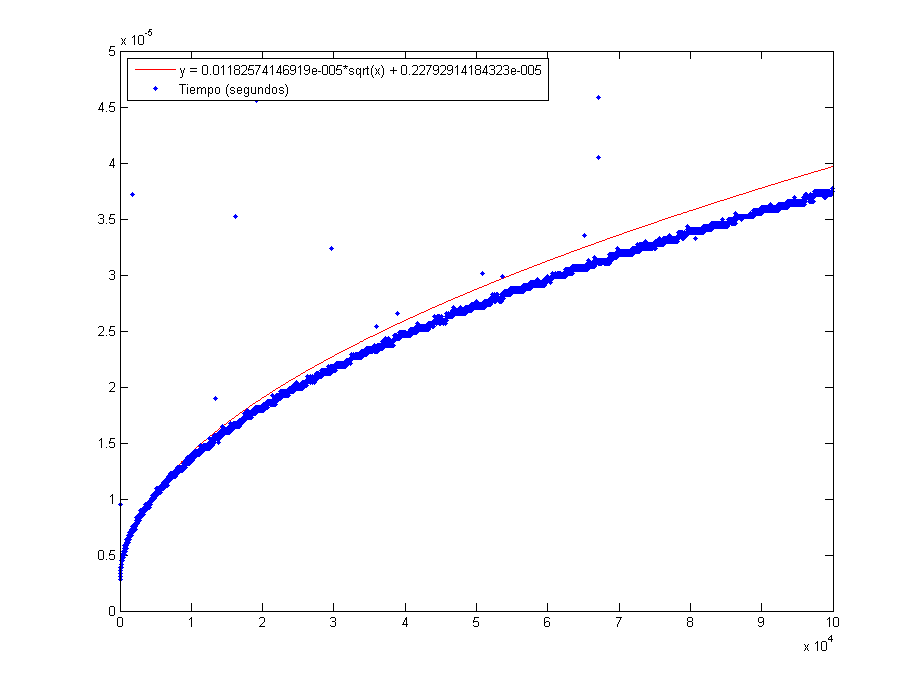
\includegraphics[scale=0.5]{../../codigo/ejercicio1/benchmark_de_tiempo/graficos/primos/primosTiempo.png}
\caption{Tiempo en funcion del n'umero para n'umeros primos}
\end{figure}

\begin{figure}[H]
\centering
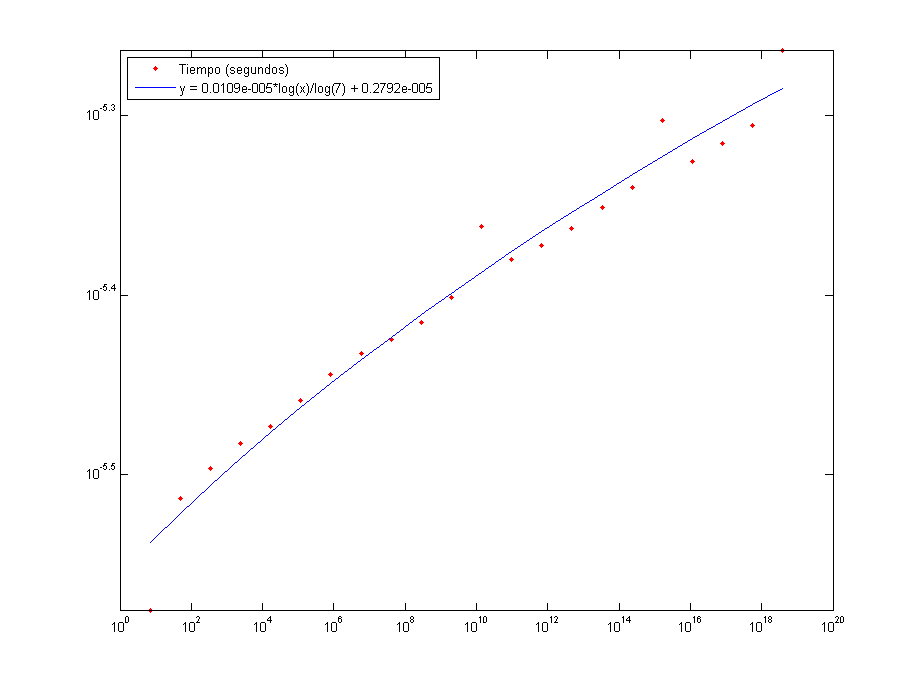
\includegraphics[scale=0.5]{../../codigo/ejercicio1/benchmark_de_tiempo/graficos/potencias_de_7/Potencias_de_7_tiempo.png}
\caption{Tiempo en funcion del n'umero para n'umeros de la forma $7^k$}
\end{figure}

\section{Discusi'on}


